\section{Auswertung}
\label{sec:Auswertung}
\subsection{Volumina und Dichten}
Zuerst wurden die Dichten $\rho_{kl}$ und $\rho_{gr}$ der kleinen und großen Kugeln bestimmt. Dazu wurden Massen
$m_{kl} = 4.453\unit{\gram}$ und $m_{gr} = 4.953 \unit{\gram}$, sowie deren gemessener Durchmesser verwendet und
damit erst die Volumina mit $V = \frac{1}{6}\pi\left(d\right)^3$ berechnet:
\begin{align*}
  V_{kl} &= \frac{1}{6}\pi\left(1.55\unit{\centi\meter}\right)^3 \approx 1.9498\unit{\cubic\centi\meter}\\
  V_{gr} &= \frac{1}{6}\pi\left(1.58\unit{\centi\meter}\right)^3 \approx 2.0652\unit{\cubic\centi\meter}.
\end{align*}
Anschließend wurden mit der Formel: $\rho = \frac{m}{V}$ die Dichten der Kugeln berechnet:
\begin{align*}
  \rho_{kl} &= \frac{m_{kl}}{V_{kl}} \approx 2.2838\unit{\gram\per\cubic\centi\meter}\\
  \rho_{gr} &= \frac{m_{gr}}{V_{gr}} \approx 2.3983\unit{\gram\per\cubic\centi\meter}
\end{align*}
\subsection{Fehlerformeln}
\begin{align*}
  \bar{x} &= \frac{1}{N}\sum_{k=1}^{N} x_k\\
  \symup{\Delta}\bar{x} &= \sqrt{\frac{1}{N\left(N-1\right)}\sum_{k=1}^{N}\left(x_k-\bar{x}\right)^2} = \sqrt{\bar{x^2}-\bar{x}^2}.
\end{align*}
Für die Berechnung der Fehlerfortpflanzung wurde die Gauß´schen Fehlerfortpflanzung verwendet:
\begin{equation*}
  \symup{\Delta}f = \sqrt{\left(\frac{\partial f}{\partial x}\symup{\Delta}x\right)^2 + \left(\frac{\partial f}{\partial y}\symup{\Delta}y\right)^2 +\ldots}
\end{equation*}
\subsection{Bestimmung der Apperatkonstanten}
Dann wurden der Mittelwert und die Standardabweichungen der Fallzeiten der Kugeln berechnet.\\
Für die kleine Kugel ergibt sich:
\begin{align*}
  \bar{t}_{hin} &=(6.197\pm 0.256)\unit{\second}\\
  \bar{t}_{zur} &=(6.324\pm 0.208)\unit{\second}.
\end{align*}
Für die große Kugel ergibt sich:
\begin{align*}
  \bar{t}_{hin} &=(40.984\pm 0.184)\unit{\second}\\
  \bar{t}_{zur} &=(40.906\pm 0.510)\unit{\second}.
\end{align*}
Nun wurde mit \eqref{} und der Apperatkonstante $K_{kl} = 0.0764\unit{\milli\pascal\cubic\centi\meter\per\gram}$
der kleinen Kugel die dynamische Viskosität $\eta$ berechnet, wobei die angegebene Apperatkonstante sich auf die Strecke
$\symup{\Delta}s = 100\unit{\milli\meter}$ bezieht, aber die Messdaten auf einer Strecke von $\symup{\Delta}s = 50\unit{\milli\meter}$ genommen wurden,
müssen die gemessenen Zeiten verdoppelt werden, hier also mit $t_{hin} = (12.394\pm 0.512)\unit{\second}$ und $t_{zur} = (12.648\pm 0.416)\unit{\second}$:
\begin{align*}
  \eta_{hin} &= (1.32575\pm 0.05477)\unit{\milli\pascal\second}\\
  \eta_{zur} &= (1.35292\pm 0.04450)\unit{\milli\pascal\second}
\end{align*}
Es wurde Gleichung \eqref{} nach $K$ umgeformt und mit dem nun bekannten $\eta$ kann $K_{gr}$ mit
den Zeiten für die große Kugel $t_{hin} = (81.968\pm 0.367)\unit{\second}$ und $t_{zur} = (81.812\pm 1.019)\unit{\second}$ berechnet werden:
\begin{align*}
  Hin : K_{gr} &= \frac{\eta_{hin}}{(\rho_K-\rho_{Fl})t_{hin}} = (11.5521\pm 0.4800)\unit{\micro\pascal\cubic\centi\meter\per\gram}\\
  Zurueck : K_{gr} &= \frac{\eta_{zur}}{(\rho_K-\rho_{Fl})t_{zur}} = (11.8113\pm 0.4154)\unit{\micro\pascal\cubic\centi\meter\per\gram}
\end{align*}
\subsection{Andradesche Gleichung}
Um die konstanten $A$ und $B$ aus der Andradeschen Gleichung zu bestimmen wurden die Werte der Messung zu verschiedenen Temperaturen aus \autoref{tab:Tabelle2}
gemittelt und die Standardabweichungen berechnet, sowie für die folgende
Berechnung die Temperaturen in $\unit{\kelvin}$ angegeben. Außerdem wurden die zugehörigen $\eta$ nach \eqref{} bestimmt.
\begin{table}[H]
  \centering
  \caption{Es wurden die Zeiten wieder verdoppelt, um sich wieder wie die Apperatkonstanten auf die Strecke von $\symup{\Delta}s=100\unit{\milli\meter}$ zu beziehen.}
  \begin{tabular}{ccccc}
    \toprule
    {$T \mathbin{/} \unit{\kelvin}$} &
    {$\bar{t}_{hin} \mathbin{/} \unit{\second}$} &
    {$\bar{t}_{zur} \mathbin{/} \unit{\second}$} &
    {$\eta_{hin} \mathbin{/} \unit{\milli\pascal\second}$} &
    {$\eta_{zur} \mathbin{/} \unit{\milli\pascal\second}$} \\
    \midrule
    298.15 & 70.34          & 70.72          & 1.1386$\pm$0.0473 & 1.1705$\pm$0.0412 \\
    302.15 & 65.15$\pm$0.25 & 67.06          & 1.0554$\pm$0.0440 & 1.1107$\pm$0.0391 \\
    305.15 & 59.61$\pm$0.31 & 59.89$\pm$0.37 & 0.9657$\pm$0.0404 & 0.9922$\pm$0.0354 \\
    307.15 & 58.73$\pm$0.49 & 58.84$\pm$0.26 & 0.9528$\pm$0.0404 & 0.9740$\pm$0.0346 \\
    309.15 & 57.16$\pm$0.42 & 57.85$\pm$0.39 & 0.9273$\pm$0.0391 & 0.9595$\pm$0.0344 \\
    311.15 & 54.31$\pm$0.59 & 55.39$\pm$0.39 & 0.8821$\pm$0.0379 & 0.9199$\pm$0.0330 \\
    313.15 & 51.7$\pm$0.26  & 52.82$\pm$0.46 & 0.8398$\pm$0.0351 & 0.8772$\pm$0.0318 \\
    315.15 & 50.82$\pm$0.02 & 50.82$\pm$0.62 & 0.8255$\pm$0.0343 & 0.8440$\pm$0.0314 \\
    317.15 & 48.61$\pm$0.53 & 48.54$\pm$0.14 & 0.7907$\pm$0.0340 & 0.8073$\pm$0.0285 \\
    319.15 & 47.34$\pm$0.26 & 47.64$\pm$0.34 & 0.7701$\pm$0.0323 & 0.7923$\pm$0.0284 \\
    321.15 & 45.59$\pm$0.43 & 45.66$\pm$0.14 & 0.7427$\pm$0.0316 & 0.7606$\pm$0.0269 \\
    323.15 & 44.2$\pm$1.24  & 44.4$\pm$0.22  & 0.7201$\pm$0.0361 & 0.7396$\pm$0.0263 \\
    \bottomrule
  \end{tabular}
  \label{tab:Tabelle3}
\end{table}
Nun wurde die Andradesche Gleichung \eqref{} so umgeformt um $\ln\left(\eta\right)$ gegen $T^{-1}$ in einem Diagramm darzustellen und dazu ein lineare Regression zu berechnen:
\begin{equation*}
  \ln\left(\eta\right) = \frac{B}{T} + \ln\left(A\right)
\end{equation*}
\begin{figure}[H]
  \centering
  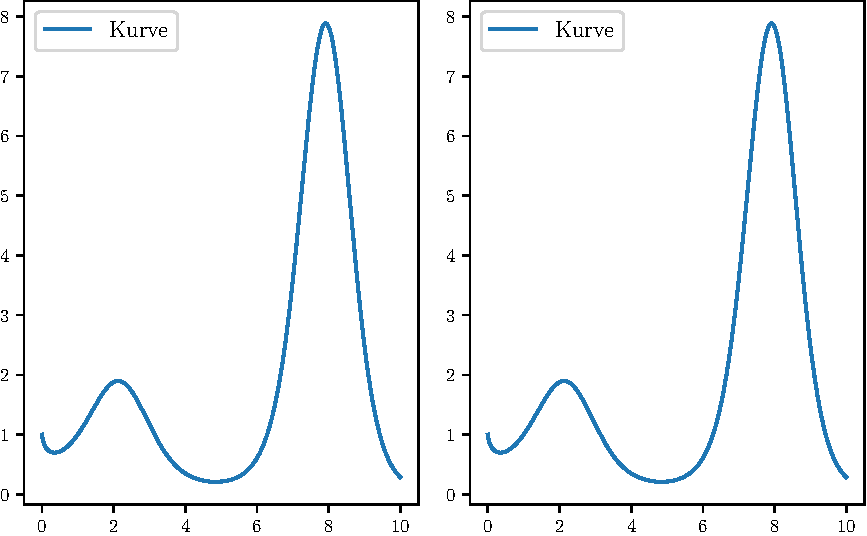
\includegraphics{plot.pdf}
  \caption{In diesem Diagramm ist $T^{-1}$ gegen $\ln\left(\eta\right)$ mit den Daten aus \autoref{tab:Tabelle3} aufgetragen, sowie die zugehörigen linearen Regressionen dargestellt.}
  \label{fig:plot}
\end{figure}
Die konstanten $A$ und $B$ der Andradeschen Gleichung ergeben sich danach für den Hinweg zu:
\begin{align*}
  \ln\left(A_{hin}\right) &= (-12.6842\pm 0.1248) \\
  A_{hin} &= (3.0997\pm 0.4120 ) \cdot 10^{-6} \\
  B_{hin} &= (1758.9033\pm 38.8663)\unit{\kelvin}.
\end{align*}
Und für den Rückweg ergibt sich:
\begin{align*}
  \ln\left(A_{zur}\right) &= (-12.7903\pm 0.1725) \\
  A_{zur} &= (2.7877\pm 0.5248 ) \cdot 10^{-6} \\
  B_{zur} &= (1801.5717\pm 53.7424)\unit{\kelvin}.
\end{align*}
Aus \autoref{fig:plot} und den berechneten Konstanten erkennt man, das die Unterteilung in hin und Rückweg nicht nötig ist, da sich die Fehlerbereiche
immer überschneiden und die Werte also nur statistische Fehler trennen.
\subsection{Reynoldsche Zahl}
Zuletzt wurde durch die Berechnung der Reynoldschen Zahl nach \eqref{} überprüft, ob es sich bei der
Strömung im Viskosimeter um eine laminare Strömung handelt. Da die Gleichung von $\farc{1}{\eta t}$ abhängt,
müssen nur deren kleinsten Werte betrachtet werden und da beide mit höheren Temperaturen sinken werden nur die Werte für
$T = 323.15\unit{\kelvin}$ bei der großen Kugel betrachtet. Da die breite des Rohres nicht gegeben ist wird Näherungsweise
der Durchmesser der großen Kugel für die charakteristische Länge verwendet:
\begin{equation*}
  Re_{gr} = 49.0455\pm 2.8176
\end{equation*}
Für die kleine Kugel ergibt sich für die Reynoldsche Zahl maximal:
\begin{equation*}
  Re_{kl} = 95.9856\pm 5.0678
\end{equation*}
Beide berechneten Reynolds Zahlen liegen deutlich unter dem Grenzwert von 2400, ab dem eine Strömung laminar wäre, daher liegt hier
keine laminare Strömung vor.